\subsection{Distributed footing: Poroelastic cube (3D)}
We consider a vertical cross-section through homogeneous soil. Due to symmetry we can limit the investigation to half of the domain. The model domain is then extending 8 meters in length and 5 meters in height. The problem is solved in 2D and 3D space, respectively.

\begin{figure}[!tbh]
\begin{center}
\scalebox{1.0} % Change this value to rescale the drawing.
{
\begin{picture}(380,190)
\put(70,160){\line(1,0){240}}
\put(310,10){\line(0,1){150}}
\multiput(70,10)(0,11){14}{\line(0,1){7}}
\put(75,180){\vector(0,-1){20}}
\put(80,180){\vector(0,-1){20}}
\put(85,180){\vector(0,-1){20}}
\put(90,180){\vector(0,-1){20}}
\put(95,180){\vector(0,-1){20}}
\put(308,165){8}
\put(60,165){0}
\put(55,8){-5}
% BC
% left
\put(5,100){$\frac{\partial p}{\partial x} = 0$}
\put(5,85) {$u_x = 0$}
\put(5,75) {$\sigma_{xy} = 0$}
% top
\put(75,150){$\sigma_{yy}=\sigma_0$}
\put(75,140){$\sigma_{xy}=0$}
\put(180,165){$\sigma_{xy}=\sigma_{yy}=0$}
\put(210,187){\vector(1,0){100}}
\put(175,187){\vector(-1,0){105}}
\put(180,185){$p=0$}
% right
\put(320,100){$\frac{\partial p}{\partial x} = 0$}
\put(320,85) {$u_x = 0$}
\put(320,75) {$\sigma_{xy} = 0$}
% bottom
\put(160,-5){$\frac{\partial p}{\partial y} = 0$ , $u_x=u_y=0$}
\linethickness{2pt}
\put(70,10){\line(1,0){240}}
\end{picture}
}
\end{center}
\caption{Conceptualization of the footing problem. Properties are Young's modulus, $E=3\times 10^{4}$ $N/m^{2}$, Poisson's ratio, $\nu =0.2$, permeability, $k=10^{-10}$ $m^2$, and fluid viscosity, $\mu =10^{-3}$ $Pa\,s$.}
\label{fig-setting}
\end{figure} 

\subsubsection*{Definition}
A strip loading is imposed ($\sigma _{yy}=\sigma _0$ in $x\in [0,1]$), with zero stresses
($\sigma _{yy}=\sigma _{xy}=0$ in $x\in(1,8]$) and zero pressure at the top; no horizontal flux, no horizontal displacements and zero shear stresses at left and right boundaries with no vertical flux and no displacement at the bottom (Fig. \ref{fig-setting}). 

\subsubsection*{Results}
The 3D geometry expands the 2D domain by extruding the 2D shape by 1m in the off-plane direction (\ref{fig_HM3}). Results at the critical step, i.e., the first step, are shown in Fig. \ref{fig:e10}, \ref{fig:e12} and  \ref{fig:e11}. The results produced using the 2D model with triangular elements and the 3D model with tetrahedral elements match each other well, thus providing confidence in higher dimensions.

\begin{figure}[!tbh]
\vspace{-1cm}
\begin{center}
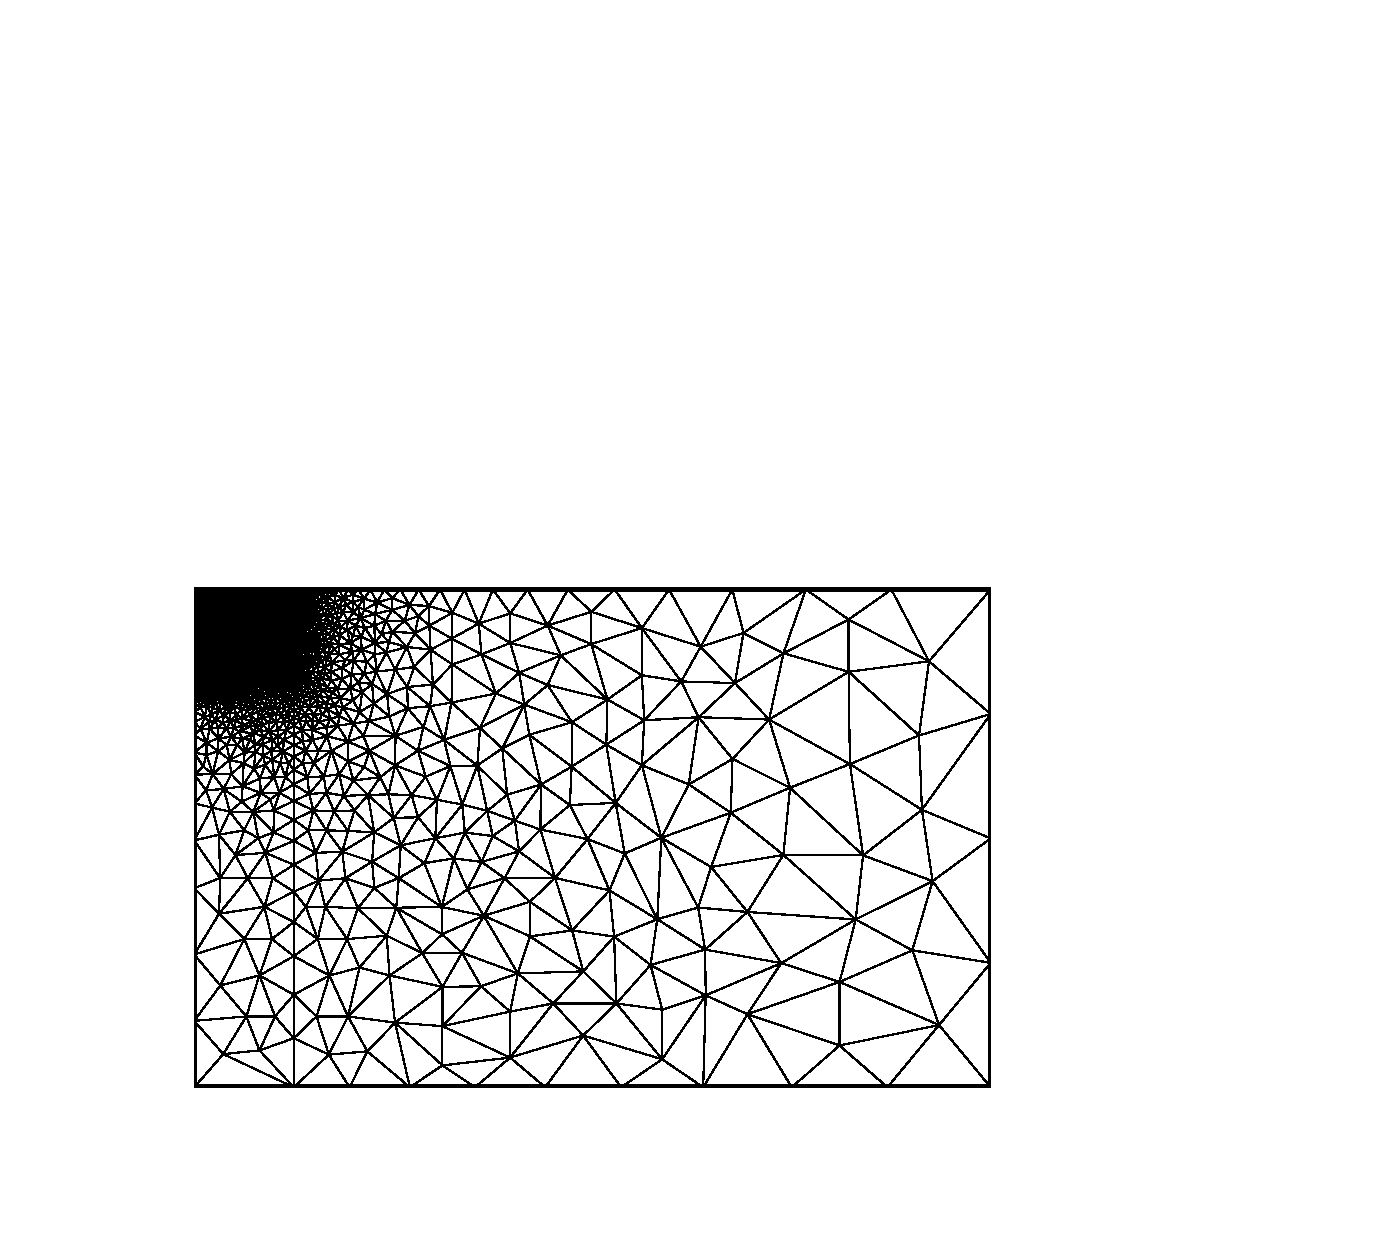
\includegraphics[width=0.54\textwidth]{chapter_14/figures/fig_14_1_4_a}
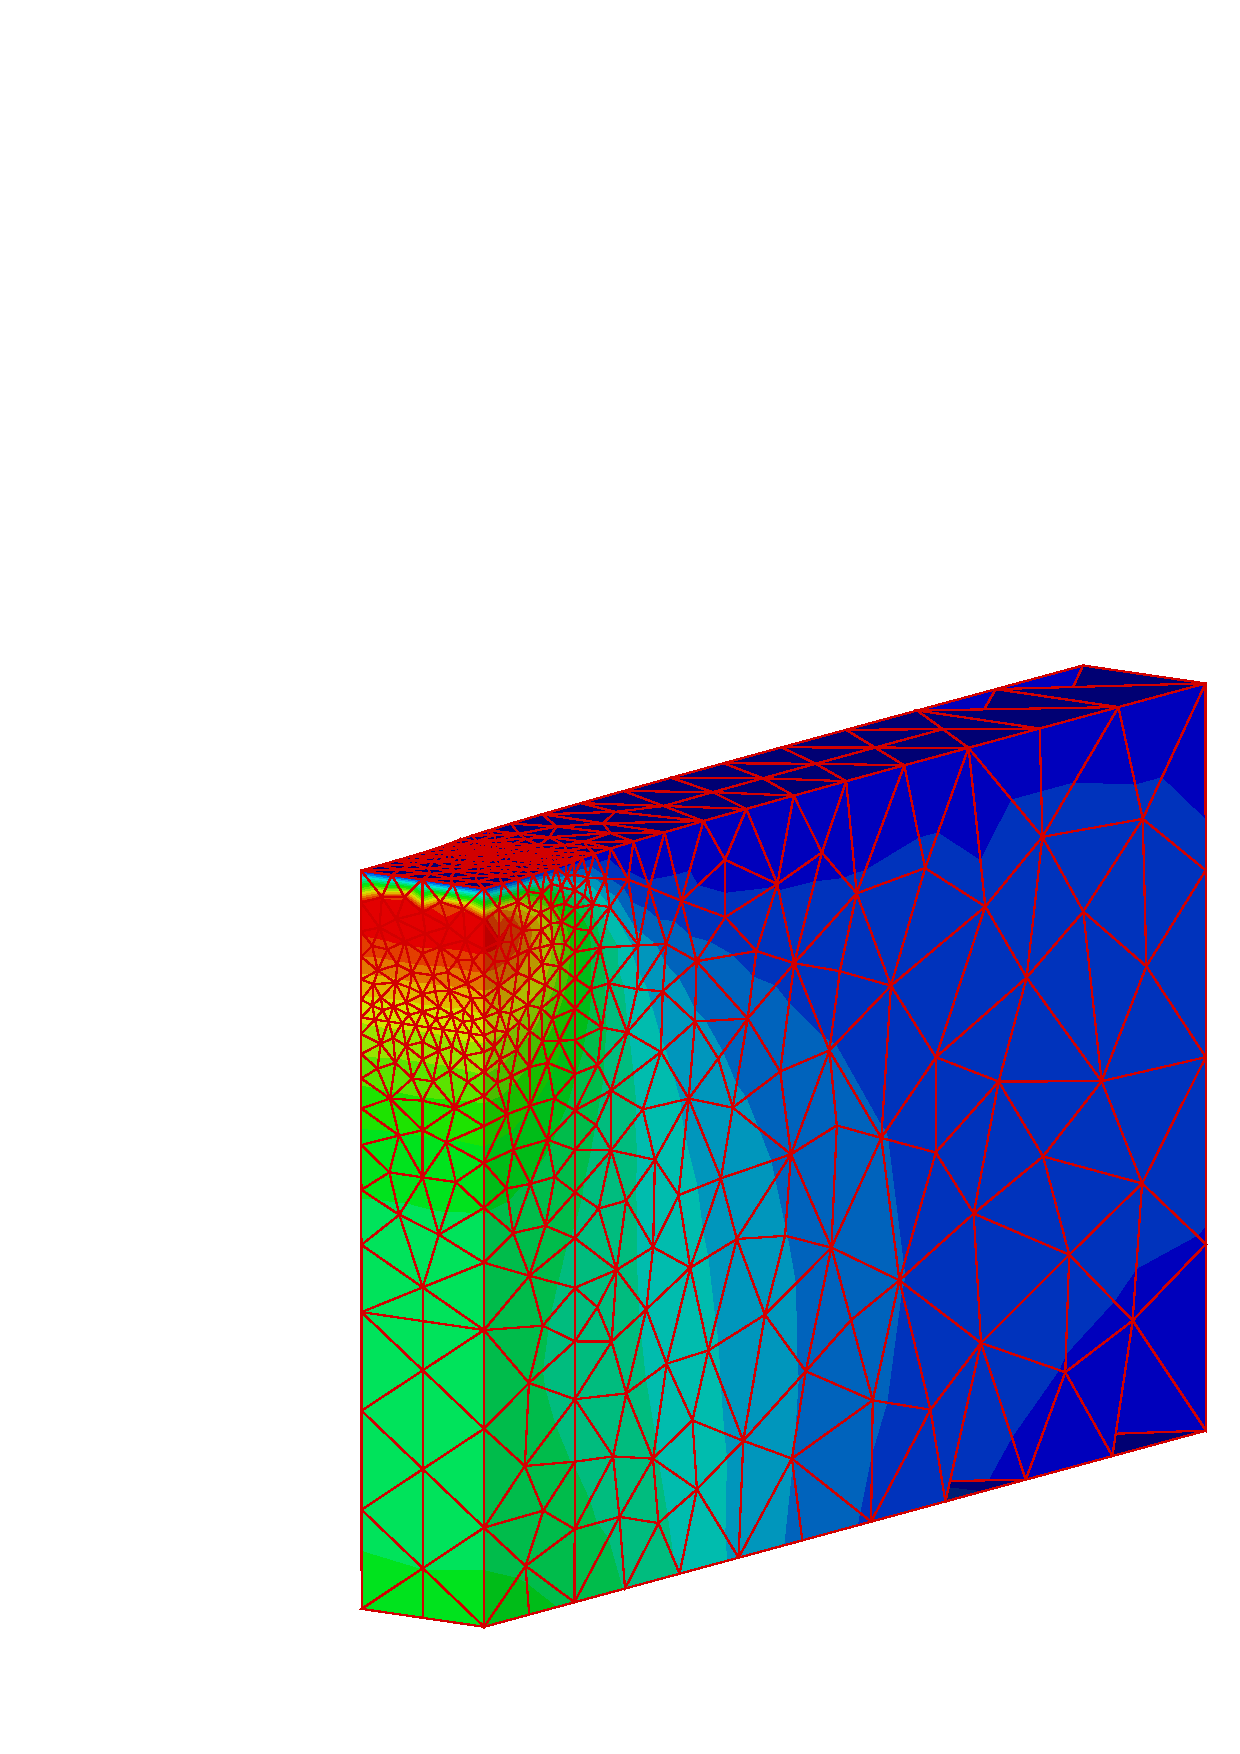
\includegraphics[width=0.44\textwidth]{chapter_14/figures/fig_14_1_4_b}
\end{center}
\vspace{-0.5cm}
\caption{Mesh geometry.}
\label{fig_HM3}
%\vspace{-1.0cm}
\end{figure}

\begin{figure}[!tbh]
\begin{center}
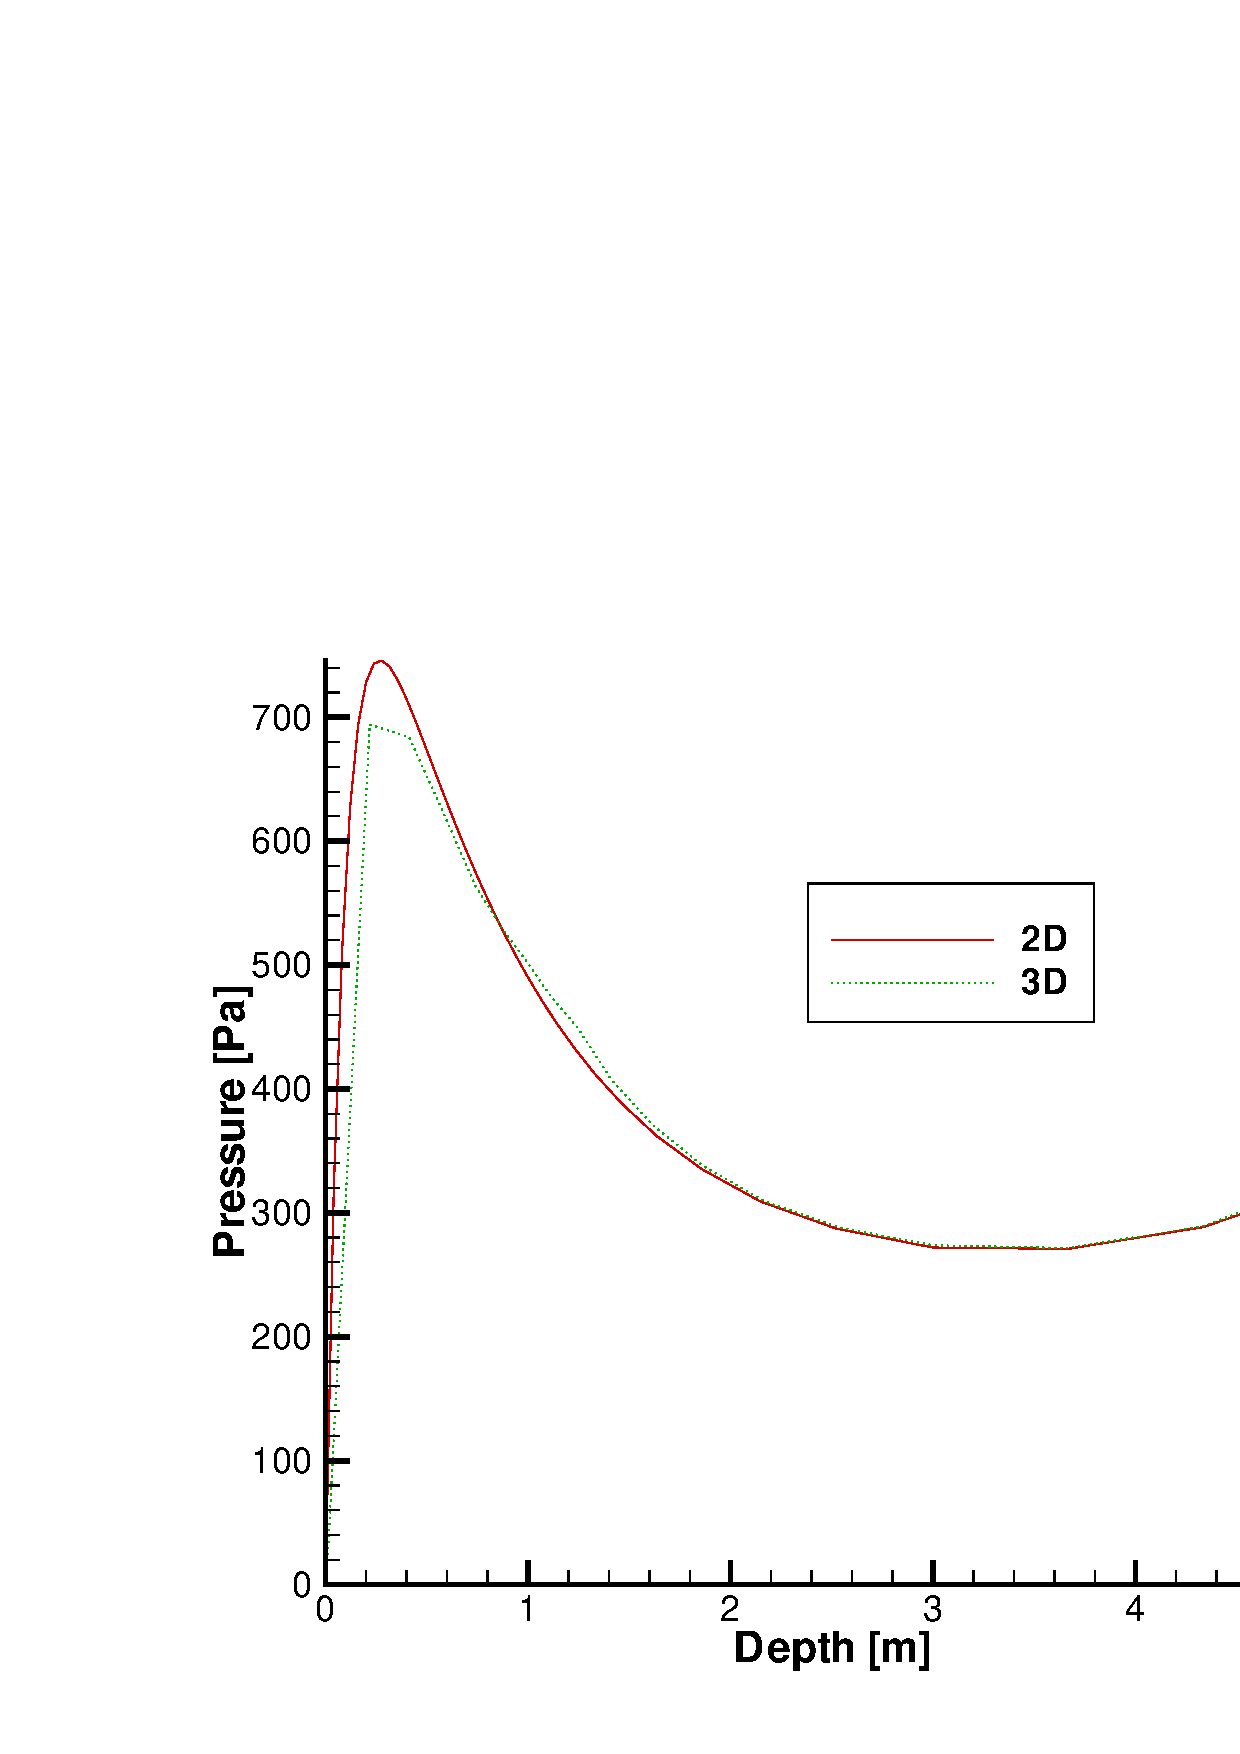
\includegraphics[width=0.49\textwidth]{chapter_14/figures/fig_14_1_5_a}
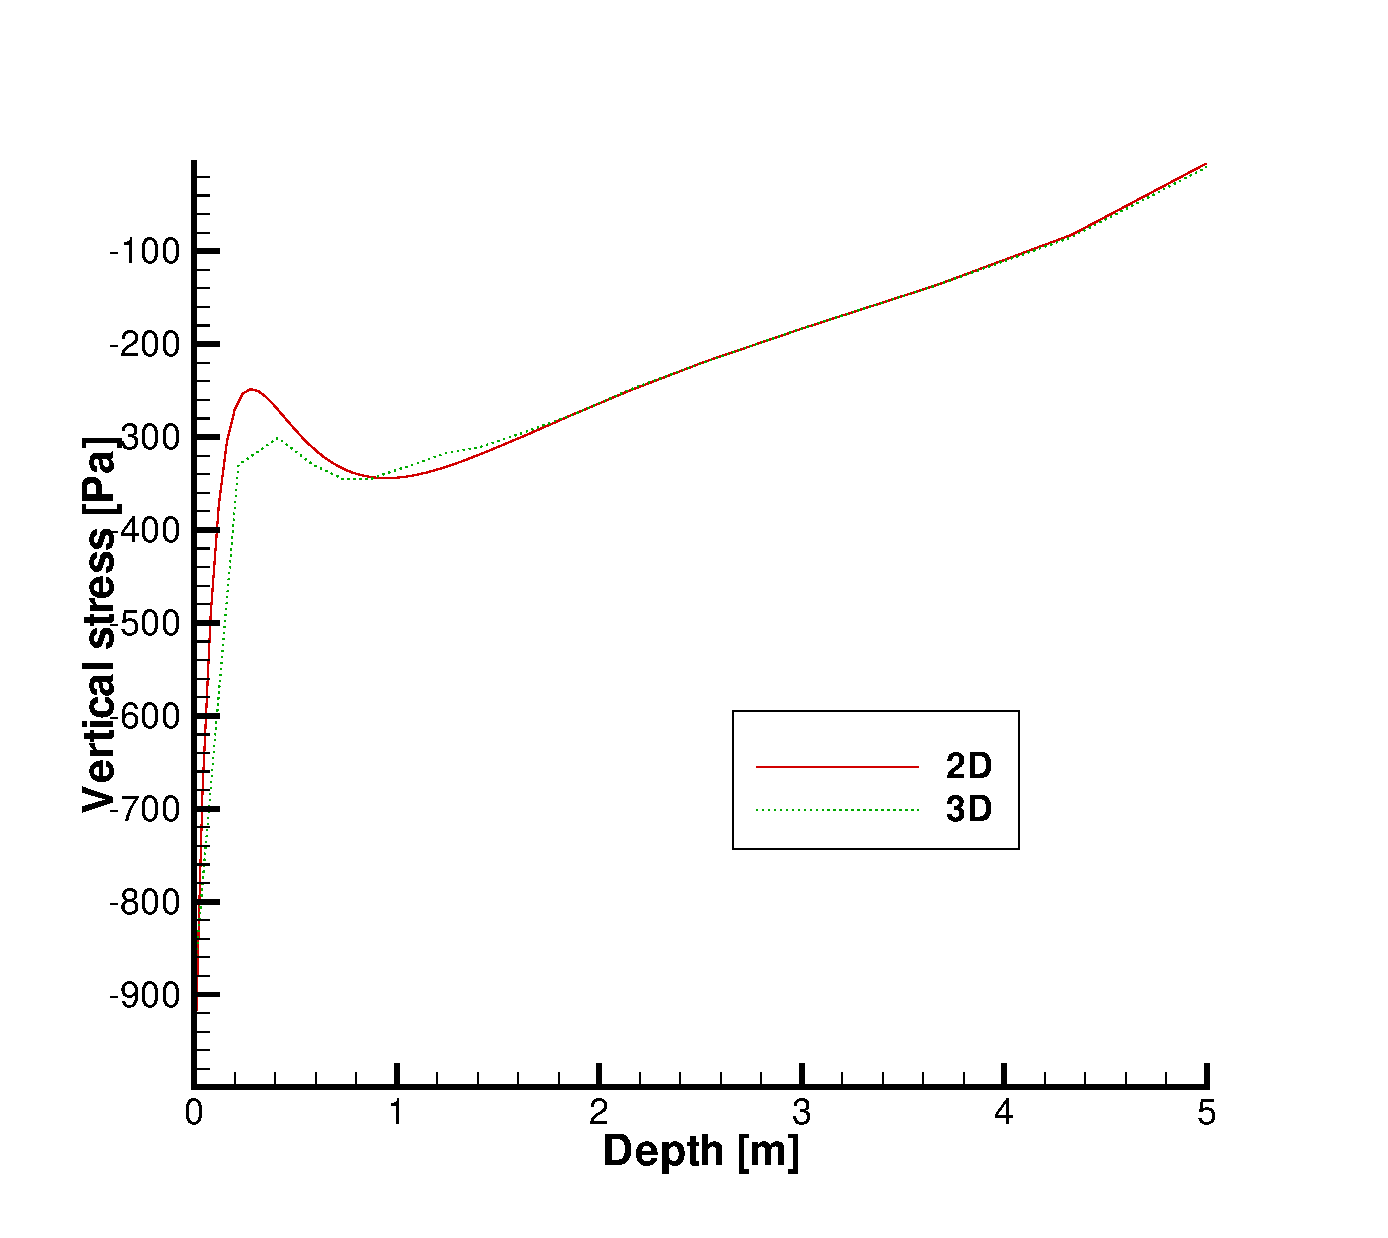
\includegraphics[width=0.49\textwidth]{chapter_14/figures/fig_14_1_5_b}
\end{center}
\caption{Comparison along symmetric axis.}  
\label{fig:e11}
\end{figure}

\begin{figure}[!tbh]
\begin{center}
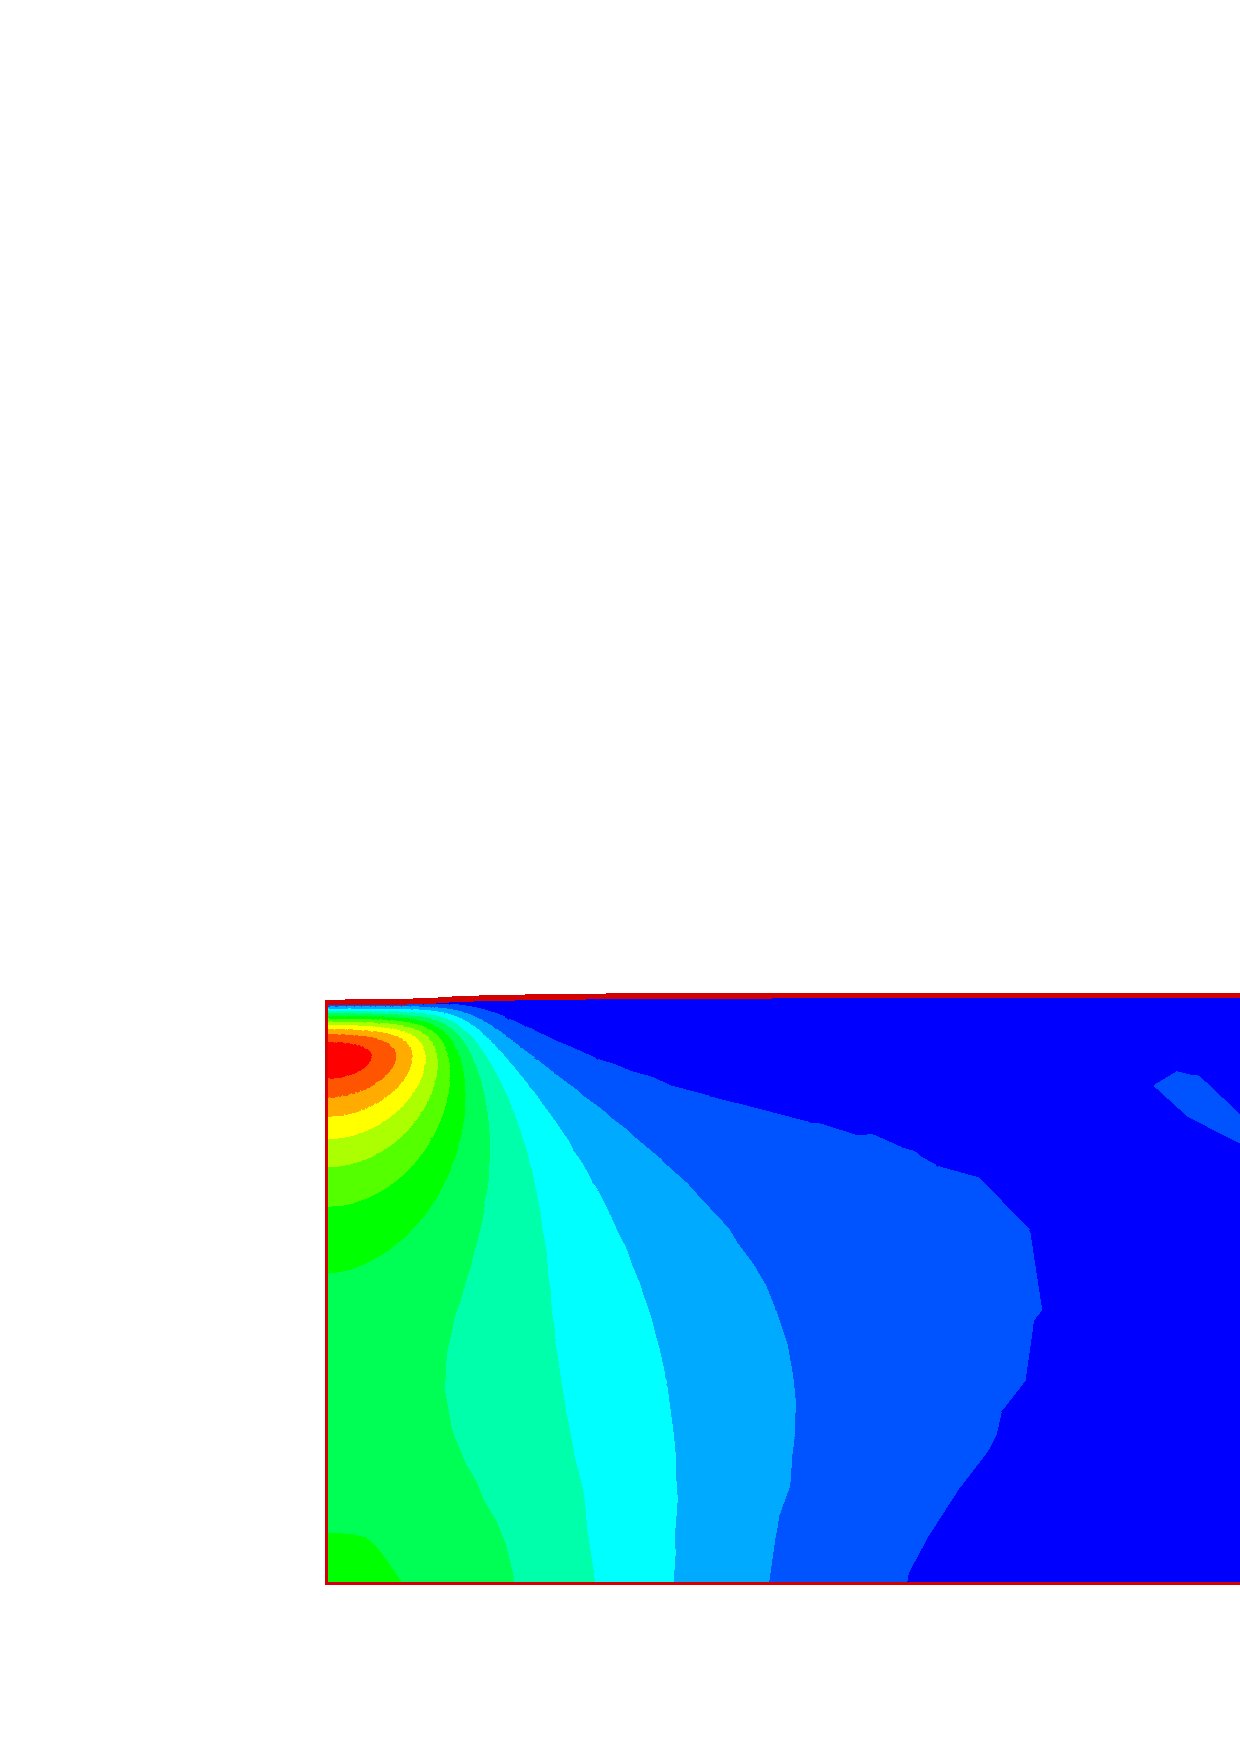
\includegraphics[width=0.49\textwidth]{chapter_14/figures/fig_14_1_6_a}
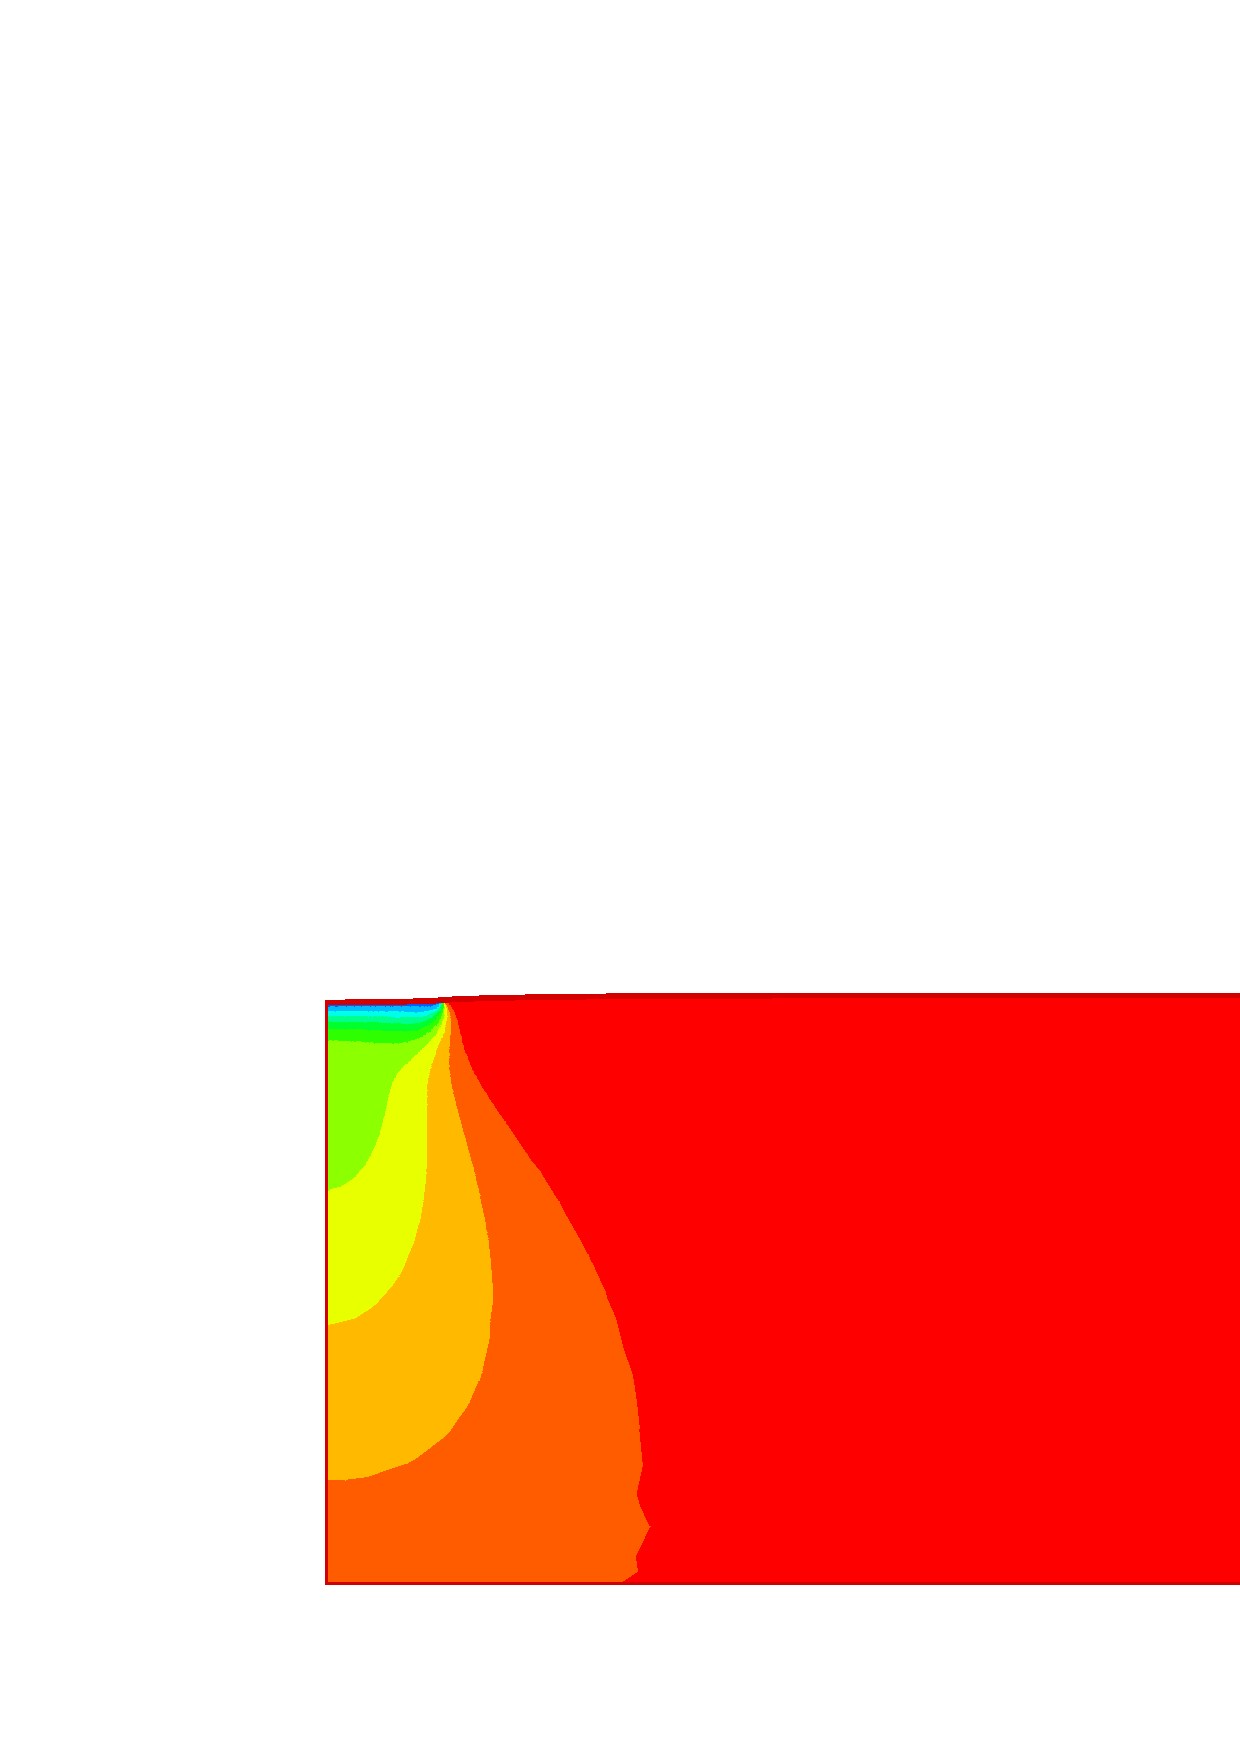
\includegraphics[width=0.49\textwidth]{chapter_14/figures/fig_14_1_6_b}
\end{center}
\vspace{-0.5cm}
\caption{2D contours.}
\label{fig:e10}

\begin{center}
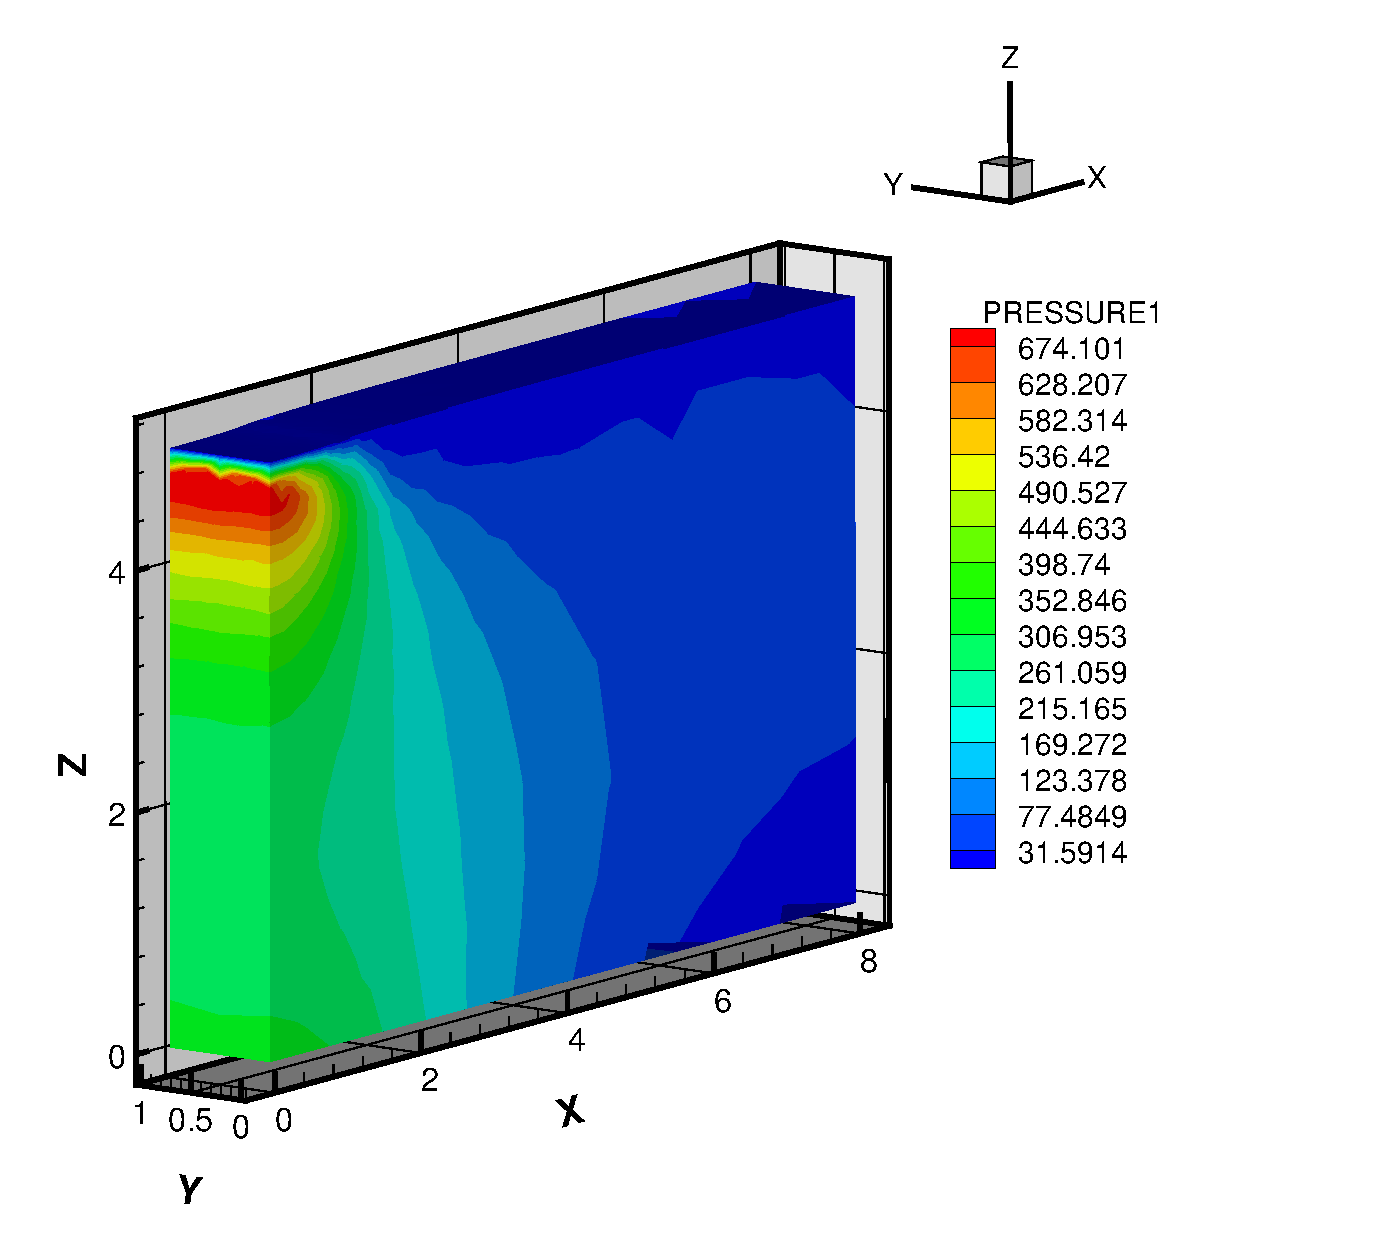
\includegraphics[width=0.49\textwidth]{chapter_14/figures/fig_14_1_7_a}
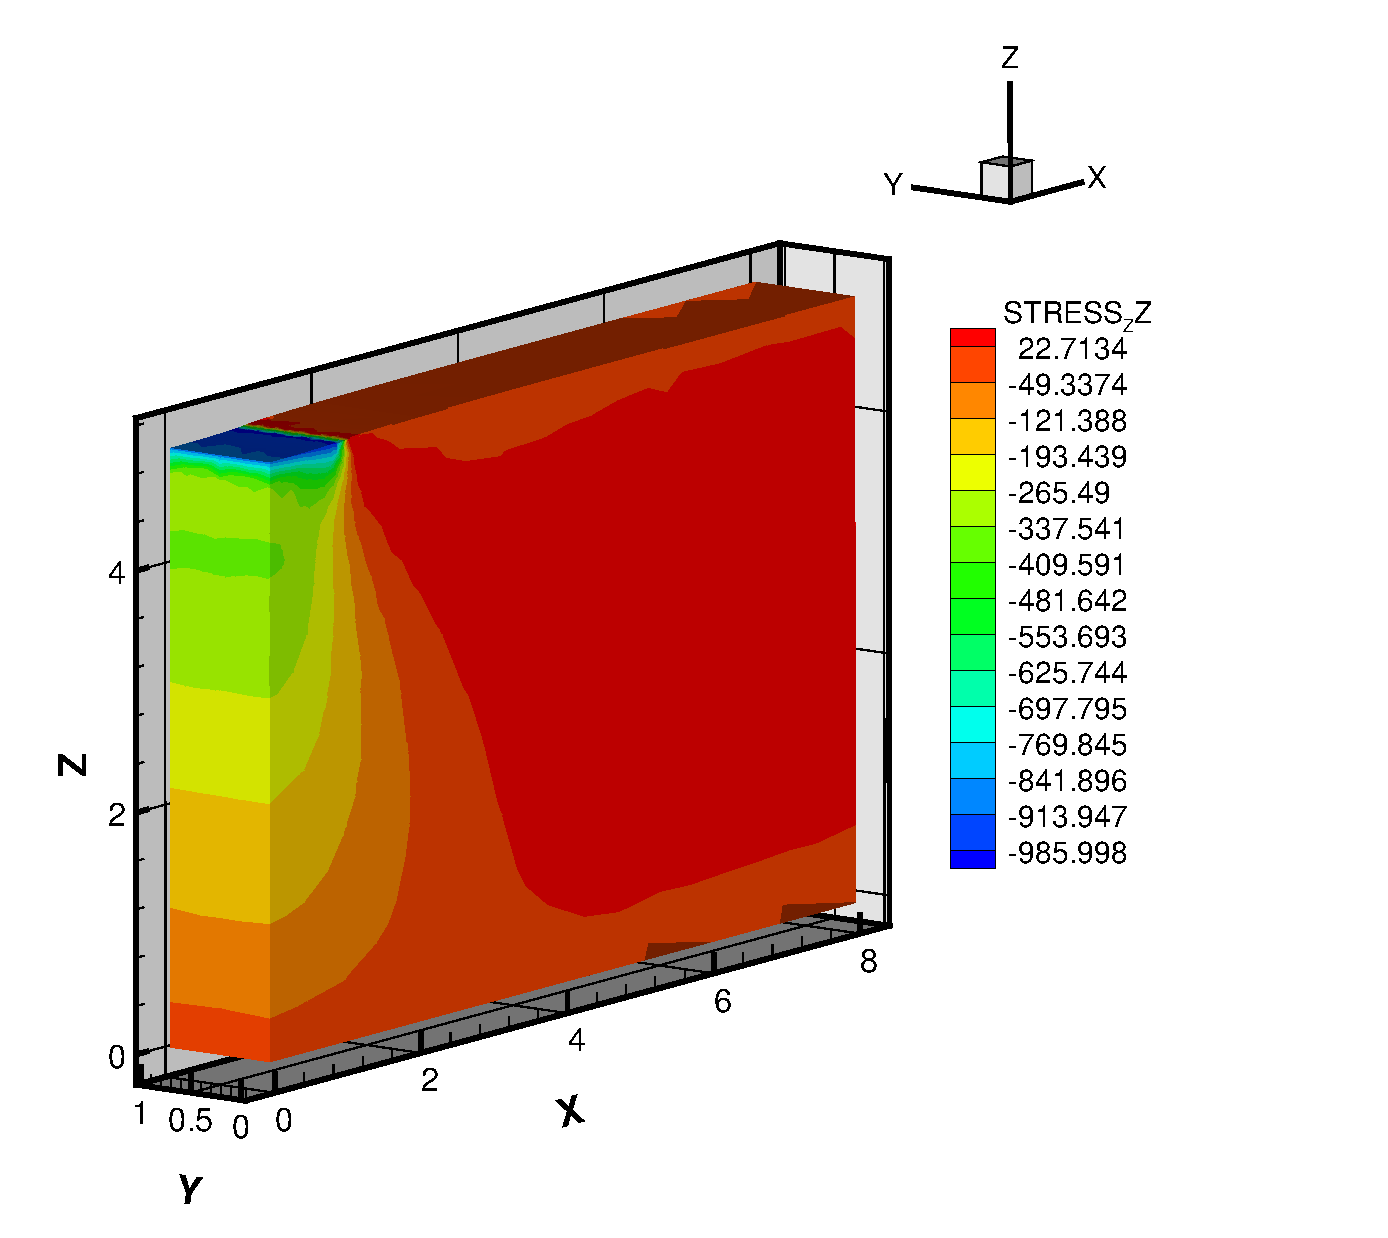
\includegraphics[width=0.49\textwidth]{chapter_14/figures/fig_14_1_7_b}
\end{center}
\vspace{-0.5cm}
\caption{3D contours.}
\label{fig:e12}
\end{figure}